% ====================================================================
%  徐森林、薛春华《数学分析》（第一册）
%  \S3.3  微分中值定理
%  源：原书印刷页 185-198（PDF 物理页 191-204）
%  底本：PaddleOCR-VL-1.6 + 高清影印比对校订
%  规范：全西文半角标点；单一落盘出口 _texout.py
% ====================================================================
\section{微分中值定理}\label{sec:3.3}

这一节主要讨论微分学中重要的 Fermat 定理、Rolle 定理、Lagrange 中值定理以及 Cauchy 中值定理, 它们是研究函数的增减性、凹凸性、极值与最值的基础.

\begin{definition}\label{def:3.3.1}
设 $f$ 定义在区间 $I$ 上, $x_0$ 为 $I$ 的内点, 即 $\exists\delta_0>0$, s.t. $B(x_0;\delta_0)=(x_0-\delta,x_0+\delta)\subset I$. 如果 $x_0$ 有一个开邻域 $B(x_0;\delta)=(x_0-\delta,x_0+\delta)\subset I$, s.t. $f(x_0)$ 为 $f(x)$ 在 $(x_0-\delta,x_0+\delta)$ 中的最大(小)值, 即 $f(x)\leqslant f(x_0)$ ($f(x)\geqslant f(x_0)$), 则称 $f(x_0)$ 为 $f$ 的极大(小)值, $x_0$ 称为 $f$ 的极大(小)值点. 极大值与极小值统称为极值. 极大值点与极小值点统称为极值点.
\end{definition}

如果 $x_0$ 为 $I$ 中的内点, 且为 $f$ 的最大(小)值点, 显然, $x_0$ 为 $f$ 的极大(小)值点. 但是, 反之不一定成立. 例如:
\[
f(x)=\begin{cases}x+1,&-2<x\leqslant0,\\ -x+1,&0<x\leqslant1,\\ 2x-2,&1<x\leqslant2,\end{cases}
\]
$x=0$ 为极大值点但非最大值点, $x=1$ 为极小值点但非最小值点.

注意, 最大(小)值若在区间端点达到, 则它就不是极大(小)值.

极值是局部性质, 而最值是整体性质.

\begin{theorem}[Fermat (1601---1665) 定理]\label{thm:3.3.1}
设 $f$ 在点 $x_0$ 处可导, $x_0$ 为 $f$ 的极值点, 则 $f'(x_0)=0$. 但反之不一定成立.
\end{theorem}

若 $f'(x_0)=0$, 则 $x_0$ 称为 $f$ 的驻点或稳定点.

\begin{proof}
不妨设 $x_0$ 为 $f$ 的极大值点, 即 $\exists\delta>0$, s.t. $f(x)\leqslant f(x_0)$, $\forall x\in(x_0-\delta,x_0+\delta)$. 于是(如图~\ref{fig:3.3.1} 所示),
\[
\frac{f(x)-f(x_0)}{x-x_0}\begin{cases}\geqslant0,&x_0-\delta<x<x_0,\\ \leqslant0,&x_0<x<x_0+\delta.\end{cases}
\]
又因为 $f$ 在点 $x_0$ 处可导, 故
\[
\begin{aligned}
0 &\leqslant\lim_{x\to x_0^-}\frac{f(x)-f(x_0)}{x-x_0}=f'_-(x_0)=f'(x_0)=f'_+(x_0)\\
&=\lim_{x\to x_0^+}\frac{f(x)-f(x_0)}{x-x_0}\leqslant0,
\end{aligned}
\]
\[
f'(x_0)=0.
\]
\end{proof}

建议读者用反证法证明 $f'(x_0)=0$.

反之有反例: $f(x)=x^{3}$, $f'(x)=3x^{2}$, $f'(0)=0$, $0$ 为 $f$ 的驻点, 但由 $f$ 严格增与反证法知, $0$ 不是 $f$ 的极值点.

\begin{remark}\label{rem:3.3.1}
定理~\ref{thm:3.3.1} 中, “可导”条件不能删去.

反例: $y=f(x)=|x|$, 显然 $0$ 为 $f$ 的极小值点(也是最小值点), 但由于 $f$ 在点 $0$ 处不可导, 当然谈不上 $f'(0)=0$.
\end{remark}

\begin{figure}[htbp]
\centering
\begin{tikzpicture}[scale=1.0,>=stealth,font=\small]
  \draw[->] (-1.60,0) -- (6.55,0) node[below right] {$x$};
  \draw[->] (0,-0.85) -- (0,5.70) node[left] {$y$};
  \node[below left] at (0,0) {$O$};
  % 水平切线 y = f(x_0)
  \draw[thick] (-1.25,3.30) -- (4.80,3.30);
  \node[left] at (-1.28,3.30) {$f(x_0)$};
  % 曲线 y = f(x)
  \draw[thick] (0.94,1.88) .. controls (1.55,2.42) and (2.35,3.23) .. (3.06,3.23)
               .. controls (3.85,3.23) and (4.72,2.52) .. (5.61,1.84);
  % 三条竖直虚线
  \draw[dashed] (1.33,3.30) -- (1.33,-1.12);
  \draw[dashed] (2.99,3.30) -- (2.99,-1.12);
  \draw[dashed] (4.80,3.30) -- (4.80,-0.52);
  % 横轴标签
  \node[below] at (1.33,-1.16) {$x_0-\delta$};
  \node[below] at (2.99,-1.16) {$x_0$};
  \node[below] at (4.80,-0.56) {$x_0+\delta$};
\end{tikzpicture}
\caption{}\label{fig:3.3.1}
\end{figure}

\begin{theorem}[Rolle (1652---1719) 定理]\label{thm:3.3.2}
设 $f$ 在 $[a,b]$ 上连续, 在 $(a,b)$ 内可导, $f(a)=f(b)$, 则 $\exists\xi\in(a,b)$, s.t. $f'(\xi)=0$ (即 $(\xi,f(\xi))$ 或 $\xi$ 点处的切线平行于 $x$ 轴, 也平行于 $(a,f(a))$ 与 $(b,f(b))$ 的连线).
\end{theorem}

\begin{proof}
因为 $f$ 在 $[a,b]$ 上连续, 由最值定理知, $f$ 必达到最大值与最小值, 即 $\exists\alpha,\beta\in[a,b]$, s.t. $f(\alpha)\leqslant f(x)\leqslant f(\beta)$, $\forall x\in[a,b]$.

如果 $\alpha,\beta\in\{a,b\}$, 则由 $f(a)=f(b)$ 知, $f(x)=f(a)=f(b)$, $\forall x\in[a,b]$, 即 $f$ 为 $[a,b]$ 上的常值函数. 于是, $\forall\xi\in(a,b)$, $f'(\xi)=0$.

如果 $\alpha,\beta$ 中有一个不是端点, 例如 $\alpha\in(a,b)$, 则由 $f$ 在 $\alpha$ 达到最小值, 它必为极小值, 由 Fermat 定理知, $f'(\alpha)=0$. 因此, $\xi=\alpha$ 为定理所求之点.
\end{proof}

\begin{theorem}[Lagrange (1736---1813) 中值定理]\label{thm:3.3.3}
设 $f$ 在 $[a,b]$ 上连续, 在 $(a,b)$ 内可导, 则 $\exists\xi\in(a,b)$, s.t.
\[
f'(\xi)=\frac{f(b)-f(a)}{b-a}
\]
($(\xi,f(\xi))$ 点处的切线平行 $(a,f(a))$ 与 $(b,f(b))$ 的连线) 或
\[
\begin{aligned}
f(b)-f(a)&=f'(\xi)(b-a)\\
&=f'[a+\theta(b-a)](b-a),
\end{aligned}
\]
其中 $0<\theta=\frac{\xi-a}{b-a}<1$.
\end{theorem}

\begin{figure}[htbp]
\centering
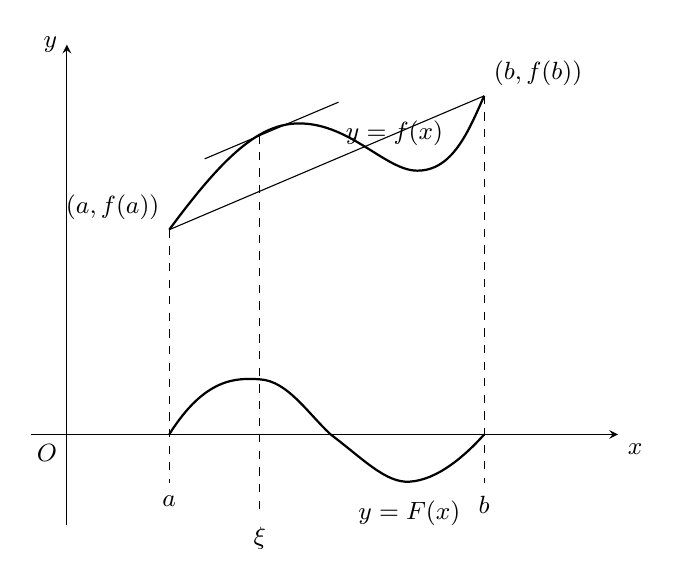
\begin{tikzpicture}[scale=1.0,>=stealth,font=\small]
  \draw[->] (-0.45,0) -- (7.00,0) node[below right] {$x$};
  \draw[->] (0,-1.15) -- (0,4.95) node[left] {$y$};
  \node[below left] at (0,0) {$O$};
  % 曲线 y = f(x)
  \draw[thick] (1.30,2.60) .. controls (2.00,3.55) and (2.45,3.95) .. (2.95,3.95)
               .. controls (3.60,3.95) and (4.05,3.35) .. (4.45,3.35)
               .. controls (4.90,3.35) and (5.10,3.85) .. (5.30,4.30);
  % 弦 (a,f(a)) -- (b,f(b))
  \draw (1.30,2.60) -- (5.30,4.30);
  % 平行于弦的切线 (过 xi 处切点)
  \draw (1.75,3.50) -- (3.45,4.22);
  % 辅助函数 y = F(x)
  \draw[thick] (1.30,0) .. controls (1.75,0.72) and (2.15,0.72) .. (2.45,0.70)
               .. controls (2.80,0.68) and (3.05,0.28) .. (3.35,0.00)
               .. controls (3.75,-0.30) and (4.05,-0.62) .. (4.35,-0.60)
               .. controls (4.70,-0.58) and (5.05,-0.28) .. (5.30,0.00);
  % 三条竖直虚线
  \draw[dashed] (1.30,2.60) -- (1.30,-0.62);
  \draw[dashed] (2.45,3.80) -- (2.45,-1.02);
  \draw[dashed] (5.30,4.30) -- (5.30,-0.62);
  % 标注
  \node[above left] at (1.30,2.60) {$(a,f(a))$};
  \node[above right] at (5.30,4.30) {$(b,f(b))$};
  \node[right] at (3.42,3.82) {$y=f(x)$};
  \node[below] at (4.35,-0.72) {$y=F(x)$};
  \node[below] at (1.30,-0.66) {$a$};
  \node[below] at (2.45,-1.06) {$\xi$};
  \node[below] at (5.30,-0.66) {$b$};
\end{tikzpicture}
\caption{}\label{fig:3.3.2}
\end{figure}

当 $f(a)=f(b)$ 时, $f'(\xi)=\frac{f(b)-f(a)}{b-a}=0$. 因此, Lagrange 中值定理为 Rolle 定理的推广.

\begin{proof}[证法 1]
从图~\ref{fig:3.3.2} 想到令
\[
F(x)=f(x)-\left[f(a)+\frac{f(b)-f(a)}{b-a}(x-a)\right],
\]
则由 $f$ 在 $[a,b]$ 上连续, 在 $(a,b)$ 上可导知, $F$ 在 $[a,b]$ 上连续, 在 $(a,b)$ 上可导, 且
\[
\begin{aligned}
F(a)&=f(a)-\left[f(a)+\frac{f(b)-f(a)}{b-a}(a-a)\right]=0\\
&=f(b)-\left[f(a)+\frac{f(b)-f(a)}{b-a}(b-a)\right]=F(b).
\end{aligned}
\]
根据 Rolle 定理可得, $\exists\xi\in(a,b)$, s.t.
\[
0=F'(\xi)=f'(\xi)-\frac{f(b)-f(a)}{b-a},
\]
\[
f'(\xi)=\frac{f(b)-f(a)}{b-a}.
\]
\end{proof}

\begin{proof}[证法 2]
令
\[
\begin{aligned}
F(x)&=\begin{vmatrix}1&a&f(a)\\1&b&f(b)\\1&x&f(x)\end{vmatrix}=\begin{vmatrix}1&a&f(a)\\0&b-a&f(b)-f(a)\\0&x-a&f(x)-f(a)\end{vmatrix}\\
&=(b-a)[f(x)-f(a)]-(x-a)[f(b)-f(a)],
\end{aligned}
\]
则由 $f$ 在 $[a,b]$ 上连续, 在 $(a,b)$ 内可导知, $F$ 在 $[a,b]$ 上连续, 在 $(a,b)$ 内可导, 且
\[
F(a)=\begin{vmatrix}1&a&f(a)\\1&b&f(b)\\1&a&f(a)\end{vmatrix}=0=\begin{vmatrix}1&a&f(a)\\1&b&f(b)\\1&b&f(b)\end{vmatrix}=F(b).
\]
根据 Rolle 定理知, $\exists\xi\in(a,b)$, s.t.
\[
\begin{aligned}
0=F'(\xi)&=\begin{vmatrix}1&a&f(a)\\1&b&f(b)\\0&1&f'(x)\end{vmatrix}_{x=\xi}=\begin{vmatrix}1&a&f(a)\\0&b-a&f(b)-f(a)\\0&1&f'(\xi)\end{vmatrix}\\
&=(b-a)f'(\xi)-[f(b)-f(a)],
\end{aligned}
\]
\[
f'(\xi)=\frac{f(b)-f(a)}{b-a}.
\]
\end{proof}

\begin{theorem}[Cauchy (1789---1957) 中值定理]\label{thm:3.3.4}
设 $f$, $g$ 在 $[a,b]$ 上连续, 在 $(a,b)$ 内可导, 且 $g'(x)\neq0$, $\forall x\in(a,b)$, 则 $\exists\xi\in(a,b)$, s.t.
\[
\frac{f(b)-f(a)}{g(b)-g(a)}=\frac{f'(\xi)}{g'(\xi)}.
\]
\end{theorem}

特别地, 当 $g(x)=x$ 时, 它就是 Lagrange 中值定理. 因此, Cauchy 中值定理为 Lagrange 中值定理的推广.

\begin{proof}[证法 1]
先证 $g(b)\neq g(a)$.

用反证法. 假设 $g(b)=g(a)$, 由 Rolle 定理知, $\exists\eta\in(a,b)$, s.t. $g'(\eta)=0$, 这与 $g'(x)\neq0$, $\forall x\in(a,b)$ 矛盾. 或由 Lagrange 中值定理知, $\exists\eta\in(a,b)$, s.t. $g(b)-g(a)=g'(\eta)(b-a)\neq0$, 故 $g(b)\neq g(a)$.

仿照定理~\ref{thm:3.3.3} 证法 1, 令
\[
F(x)=f(x)-\left[f(a)+\frac{f(b)-f(a)}{g(b)-g(a)}(g(x)-g(a))\right],
\]
则由 $f$, $g$ 在 $[a,b]$ 上连续, 在 $(a,b)$ 内可导知 $F$ 在 $[a,b]$ 上连续, 在 $(a,b)$ 内可导, 且
\[
\begin{aligned}
F(a)&=f(a)-\left[f(a)+\frac{f(b)-f(a)}{g(b)-g(a)}(g(a)-g(a))\right]=0\\
&=f(b)-\left[f(a)+\frac{f(b)-f(a)}{g(b)-g(a)}(g(b)-g(a))\right]\\
&=F(b).
\end{aligned}
\]
根据 Rolle 定理可得, $\exists\xi\in(a,b)$, s.t.
\[
0=F'(\xi)=f'(\xi)-\frac{f(b)-f(a)}{g(b)-g(a)}g'(\xi),
\]
\[
\frac{f(b)-f(a)}{g(b)-g(a)}=\frac{f'(\xi)}{g'(\xi)}.
\]
\end{proof}

\begin{proof}[证法 2]
仿照定理~\ref{thm:3.3.3} 证法 2, 令
\[
F(x)=\begin{vmatrix}1&g(a)&f(a)\\1&g(b)&f(b)\\1&g(x)&f(x)\end{vmatrix},
\]
则由 $f$, $g$ 在 $[a,b]$ 上连续, 在 $(a,b)$ 内可导知, $F$ 在 $[a,b]$ 上连续, 在 $(a,b)$ 内可导, 且
\[
F(a)=\begin{vmatrix}1&g(a)&f(a)\\1&g(b)&f(b)\\1&g(a)&f(a)\end{vmatrix}=0=\begin{vmatrix}1&g(a)&f(a)\\1&g(b)&f(b)\\1&g(b)&f(b)\end{vmatrix}=F(b).
\]
根据 Rolle 定理可得, $\exists\xi\in(a,b)$, s.t.
\[
\begin{aligned}
0=F'(\xi)&=\begin{vmatrix}1&g(a)&f(a)\\1&g(b)&f(b)\\0&g'(x)&f'(x)\end{vmatrix}_{x=\xi}=\begin{vmatrix}1&g(a)&f(a)\\0&g(b)-g(a)&f(b)-f(a)\\0&g'(\xi)&f'(\xi)\end{vmatrix}\\
&=f'(\xi)[g(b)-g(a)]-g'(\xi)[f(b)-f(a)],
\end{aligned}
\]
\[
\frac{f(b)-f(a)}{g(b)-g(a)}=\frac{f'(\xi)}{g'(\xi)}.
\]
\end{proof}

\begin{corollary}\label{cor:3.3.1}
设 $f$ 在区间 $I$ 上连续, 在 $\mathring{I}$ 内可导, 则
\[
f(x)=c\ (\text{常数})\Longleftrightarrow f'(x)=0,\quad\forall x\in\mathring{I}.
\]
\end{corollary}

\begin{proof}
($\Rightarrow$) 设 $f(x)=c$, $\forall x\in\mathring{I}$, 则 $f'(x)=c'=0$.

($\Leftarrow$) $\forall x_1,x_2\in I$, $x_1<x_2$, 由 $f$ 在 $[x_1,x_2]$ 上连续, 在 $(x_1,x_2)$ 内可导, 以及 Lagrange 中值定理可知, $\exists\xi\in(x_1,x_2)\subset\mathring{I}$, s.t.
\[
\begin{aligned}
f(x_2)-f(x_1)&=f'(\xi)(x_2-x_1)=0\cdot(x_2-x_1)=0,\\
f(x_1)&=f(x_2).
\end{aligned}
\]
因为 $x_1$, $x_2$ 是任取的, 所以, $f(x)=c$ (常数).
\end{proof}

\begin{example}\label{ex:3.3.1}
设
\[
f(x)=\begin{cases}1,&x>0,\\ -1,&x<0.\end{cases}
\]
显然, $f'(x)=0$, 但 $f(x)\neq c$ (常数). 注意: $f$ 的定义域不为一个区间. 因而, 推论~\ref{cor:3.3.1} 充分性的证明中不能应用 Lagrange 中值定理.
\end{example}

\begin{corollary}\label{cor:3.3.2}
设 $f$, $g$ 在区间 $I$ 上的连续, 在 $\mathring{I}$ 内可导, 则
\[
f(x)=g(x)+c\Longleftrightarrow f'(x)=g'(x),\quad\forall x\in\mathring{I},
\]
其中 $c$ 为常数.
\end{corollary}

\begin{proof}
\[
\begin{aligned}
& f(x)=g(x)+c,\ \forall x\in I\\
\Longleftrightarrow\ & f(x)-g(x)=c,\ \forall x\in I\\
\xlongleftrightarrow{\text{推论}~\ref{cor:3.3.1}}\ & f'(x)-g'(x)=[f(x)-g(x)]'=0,\ \forall x\in\mathring{I}\\
\Longleftrightarrow\ & f'(x)=g'(x),\ \forall x\in\mathring{I}.
\end{aligned}
\]
\end{proof}

\begin{corollary}\label{cor:3.3.3}
设 $I_1$, $I_2$ 为两个不相交的非空区间. 则
\[
f(x)=\begin{cases}g(x)+c_1,&x\in I_1,\\ g(x)+c_2,&x\in I_2,\end{cases}\qquad c_1\ \text{与}\ c_2\ \text{为两个无关的常数}
\]
\[
\Longleftrightarrow f'(x)=g'(x),\quad\forall x\in\mathring{I}_1\cup\mathring{I}_2.
\]
\end{corollary}

\begin{proof}
($\Rightarrow$) 显然.

($\Leftarrow$) 因 $f'(x)=g'(x)$, $\forall x\in\mathring{I}_1\cup\mathring{I}_2$, 根据推论~\ref{cor:3.3.1} 知, $\exists c_1,c_2\in\mathbb{R}$, s.t.
\[
f(x)=\begin{cases}g(x)+c_1,&x\in I_1,\\ g(x)+c_2,&x\in I_2.\end{cases}
\]
\end{proof}

\begin{theorem}[Darboux (1842---1917) 导函数介值定理]\label{thm:3.3.5}
设 $f$ 在 $[a,b]$ 内可导, 则对于 $f'_+(a)$ 与 $f'_-(b)$ 之间的一切值 $k$, 必有 $\xi\in[a,b]$, s.t. $f'(\xi)=k$.
\end{theorem}

如果 $f'_+(a)\neq f'_-(b)$, $k\in(\min\{f'_+(a),f'_-(a)\},\max\{f'_+(a),f'_-(a)\})$, 则可取 $\xi\in(a,b)$, s.t. $f'(\xi)=k$.

\begin{proof}[证法 1]
设 $F(x)=f(x)-kx$, 由 $f$ 在 $[a,b]$ 上可导知, $F$ 在 $[a,b]$ 上也可导, 且
\[
F'_+(a)\cdot F'_-(b)=(f'_+(a)-k)(f'_-(b)-k)\leqslant0.
\]
如果 $F'_+(a)\cdot F'_-(b)=0$, 则 $F'_+(a)=0$ 或 $F'_-(b)=0$, 取 $\xi=a$ 或 $b$.

如果 $F'_+(a)\cdot F'_-(b)<0$, 不妨设
\[
\lim_{x\to a^+}\frac{F(x)-F(a)}{x-a}=F'_+(a)>0,
\]
\[
\lim_{x\to b^-}\frac{F(x)-F(b)}{x-b}=F'_-(b)<0,
\]
由保号性定理知, $\exists a_1,b_1$, s.t. $a<a_1<b_1<b$, 且
\[
F(a)<F(a_1),\quad F(b_1)>F(b).\tag*{(*)}
\]
因为 $F$ 在 $[a,b]$ 上可导, 所以它在 $[a,b]$ 上连续. 根据最值定理知, $\exists\xi\in[a,b]$, s.t. $F$ 在 $\xi$ 达到最大值. 由 $(*)$ 式知, $\xi\neq a,b$, 必有 $\xi\in(a,b)$. 因此, $\xi$ 为 $F$ 的极大值点. 再根据 Fermat 定理得到
\[
\begin{aligned}
0=F'(\xi)&=(f(x)-kx)'\big|_{x=\xi}=f'(\xi)-k,\\
f'(\xi)&=k.
\end{aligned}
\]
\end{proof}

\begin{proof}[证法 2]
设
\[
\varphi_1(x)=\begin{cases}\frac{f(x)-f(a)}{x-a},&a<x\leqslant b,\\ f'_+(a),&x=a,\end{cases}
\]
\[
\varphi_2(x)=\begin{cases}\frac{f(x)-f(b)}{x-b},&a\leqslant x<b,\\ f'_-(b),&x=b.\end{cases}
\]
因为
\[
\lim_{x\to a^+}\varphi_1(x)=\lim_{x\to a^+}\frac{f(x)-f(a)}{x-a}=f'_+(a)=\varphi_1(a),
\]
\[
\lim_{x\to b^-}\varphi_2(x)=\lim_{x\to b^-}\frac{f(x)-f(b)}{x-b}=f'_-(b)=\varphi_2(b),
\]
所以, $\varphi_1$, $\varphi_2$ 都在 $[a,b]$ 上连续, 在 $(a,b)$ 内可导.

如果 $k=f'_+(a)$, 取 $\xi=a$; 如果 $k=f'_-(b)$, 取 $\xi=b$. 如果 $f'_+(a)<k<f'_-(b)$ (或 $f'_-(b)<k<f'_+(a)$), 则 $k$ 应介于 $f'_+(a)$ 与 $\frac{f(b)-f(a)}{b-a}$ 之间或介于 $\frac{f(b)-f(a)}{b-a}$ 与 $f'_-(b)$ 之间, 不妨设为前者. 由 $\varphi_1$ 的定义知, $k$ 介于 $\varphi_1(a)$ 与 $\varphi_1(b)$ 之间. 根据 $\varphi_1$ 的连续性及连续函数的介值定理知, $\exists\theta\in[a,b]$, 由 Lagrange 中值定理知, $\exists\xi\in(a,\theta)\subset(a,b)$, s.t.
\[
k=\varphi_1(\theta)=\frac{f(\theta)-f(a)}{\theta-a}=f'(\xi).
\]
\end{proof}

\begin{remark}\label{rem:3.3.2}
注意, Darboux 定理~\ref{thm:3.3.5} 中, $f'(x)$ 不必连续. 如果 $f'$ 连续, 只需将连续函数的介值定理应用于 $f'(x)$ 即得定理~\ref{thm:3.3.5} 的结论.
\end{remark}

\begin{example}\label{ex:3.3.2}
证明: $\forall h>-1$, $h\neq0$ 成立不等式
\[
\frac{h}{1+h}<\ln(1+h)<h.
\]
\end{example}

\begin{proof}
令 $f(x)=\ln(1+x)$, 则由 Lagrange 中值定理, 有
\[
\ln(1+h)=\ln(1+h)-\ln1=\frac{h}{1+\theta h},\quad0<\theta<1.
\]
如果 $h>0$, 由 $0<\theta<1$ 推得
\[
1<1+\theta h<1+h,
\]
\[
\frac{h}{1+h}<\frac{h}{1+\theta h}<h,
\]
\[
\frac{h}{1+h}<\ln(1+h)<h.
\]
如果 $-1<h<0$, 由 $0<\theta<1$ 推得
\[
0<1+h<1+\theta h<1,
\]
\[
\frac{h}{1+h}<\frac{h}{1+\theta h}<h,
\]
\[
\frac{h}{1+h}<\ln(1+h)<h.
\]
\end{proof}

\begin{example}\label{ex:3.3.3}
设 $0<\alpha\leqslant\beta<\frac{\pi}{2}$, 证明:
\[
\frac{\beta-\alpha}{\cos^{2}\alpha}\leqslant\tan\beta-\tan\alpha\leqslant\frac{\beta-\alpha}{\cos^{2}\beta}.
\]
\end{example}

\begin{proof}
当 $\alpha=\beta$ 时, 上述不等式为等式.

当 $\alpha\neq\beta$ 时, 令 $f(x)=\tan x$, $0<\alpha\leqslant x\leqslant\beta<\frac{\pi}{2}$. 由于 $f(x)=\tan x$ 在 $[\alpha,\beta]$ 上连续, 在 $(\alpha,\beta)$ 内可导, 根据 Lagrange 中值定理知, $\exists\xi\in(\alpha,\beta)$, s.t. $\tan\beta-\tan\alpha=(\tan x)'\big|_{x=\xi}(\beta-\alpha)=\sec^{2}\xi\cdot(\beta-\alpha)=\frac{\beta-\alpha}{\cos^{2}\xi}$. 于是,
\[
\begin{aligned}
&\frac{\beta-\alpha}{\cos^{2}\alpha}<\frac{\beta-\alpha}{\cos^{2}\xi}<\frac{\beta-\alpha}{\cos^{2}\beta}.\\
&\frac{\beta-\alpha}{\cos^{2}\alpha}<\tan\beta-\tan\alpha<\frac{\beta-\alpha}{\cos^{2}\beta}.
\end{aligned}
\]
\end{proof}

\begin{example}\label{ex:3.3.4}
证明: $\arctan\frac{1+x}{1-x}=\arctan x+\frac{\pi}{4}$, $|x|<1$.
\end{example}

\begin{proof}
设 $f(x)=\arctan\frac{1+x}{1-x}-\arctan x$, $|x|<1$, 则
\[
\begin{aligned}
f'(x)&=\frac{1}{1+\left(\frac{1+x}{1-x}\right)^{2}}\cdot\frac{(1-x)+(1+x)}{(1-x)^{2}}-\frac{1}{1+x^{2}}\\
&=\frac{2}{(1-x)^{2}+(1+x)^{2}}-\frac{1}{1+x^{2}}=0,\quad|x|<1.
\end{aligned}
\]
根据推论~\ref{cor:3.3.1} 可知,
\[
\arctan\frac{1+x}{1-x}-\arctan x=f(x)=f(0)=\frac{\pi}{4}-0=\frac{\pi}{4},
\]
即
\[
\arctan\frac{1+x}{1-x}=\arctan x+\frac{\pi}{4},\quad|x|<1.
\]
\end{proof}

\begin{example}\label{ex:3.3.5}
设 $f$ 在 $[a,b]$ ($a>0$) 上连续, 在 $(a,b)$ 内可导, 则 $\exists\xi\in(a,b)$, s.t.
\[
f(b)-f(a)=\xi f'(\xi)\ln\frac{b}{a}.
\]
\end{example}

\begin{proof}
令 $g(x)=\ln x$, 显然它在 $[a,b]$ 上连续, 在 $(a,b)$ 内可导,
\[
g'(x)=(\ln x)'=\frac{1}{x}\neq0,\quad\forall x\in(a,b).
\]
由 Cauchy 中值定理, $\exists\xi\in(a,b)$, s.t.
\[
\frac{f(b)-f(a)}{\ln b-\ln a}=\frac{f'(\xi)}{\frac{1}{\xi}},
\]
即
\[
f(b)-f(a)=\xi f'(\xi)\ln\frac{b}{a}.
\]
\end{proof}

\begin{example}\label{ex:3.3.6}
设 $f:\mathbb{R}\to\mathbb{R}$ 可导. 证明: $f(x)=0$ 的任何两相异根之间必有 $f'(x)-af(x)=0$ 的一个根, 其中 $a\in\mathbb{R}$.
\end{example}

\begin{proof}
设 $x_1$, $x_2$ 为 $f(x)=0$ 的两个相异的根, 不妨设 $x_1<x_2$. 令
\[
F(x)=f(x)\mathrm{e}^{-ax},
\]
$F$ 在 $\mathbb{R}$ 上可导, 且
\[
F'(x)=\mathrm{e}^{-ax}[f'(x)-af(x)].
\]
显然,
\[
F(x_1)=f(x_1)\mathrm{e}^{-ax_1}=0=f(x_2)\mathrm{e}^{-ax_2}=F(x_2).
\]
根据 Rolle 定理知, $\exists\xi\in(x_1,x_2)$, s.t.
\[
0=F'(\xi)=\mathrm{e}^{-a\xi}[f'(\xi)-af(\xi)],
\]
即
\[
f'(\xi)-af(\xi)=0,
\]
$\xi$ 为 $f'(x)-af(x)=0$ 的一个根.
\end{proof}

\begin{example}\label{ex:3.3.7}
设 $f$ 在 $[0,a]$ 上 2 阶可导 ($a>0$), $|f''(x)|\leqslant M$, $\forall x\in[0,a]$, 且 $f$ 在 $(0,a)$ 内达到最大值. 证明: $|f'(0)|+|f'(a)|\leqslant Ma$.
\end{example}

\begin{proof}
设 $x_0\in(0,a)$, s.t. $f(x_0)=\max\limits_{0\leqslant x\leqslant a}f(x)$, 则由 Fermat 定理知, $f'(x_0)=0$. 将 Lagrange 中值定理应用于 $f'(x)$, 得: $\exists\xi_1\in(0,x_0)$, $\exists\xi_2\in(x_0,a)$, s.t.
\[
\begin{aligned}
f'(0)&=f'(x_0)+f''(\xi_1)(0-x_0)=-f''(\xi_1)x_0,\\
f'(a)&=f'(x_0)+f''(\xi_2)(a-x_0)=-f''(\xi_2)(a-x_0).
\end{aligned}
\]
因此
\[
\begin{aligned}
|f'(0)|+|f'(a)|&=|f''(\xi_1)x_0|+|f''(\xi_2)(a-x_0)|\\
&\leqslant Mx_0+M(a-x_0)=Ma.
\end{aligned}
\]
\end{proof}

\begin{example}\label{ex:3.3.8}
设 $f:\mathbb{R}\to\mathbb{R}$ 2 阶可导, $|f(x)|\leqslant1$, 且
\[
[f(0)]^{2}+[f'(0)]^{2}=4.
\]
证明: $\exists\xi\in(-2,2)$, s.t. $f(\xi)+f''(\xi)=0$.
\end{example}

\begin{proof}
令 $F(x)=[f(x)]^{2}+[f'(x)]^{2}$, 则
\[
F'(x)=2f'(x)[f(x)+f''(x)].
\]
由 Lagrange 中值定理知, $\exists a\in(-2,0)$, $b\in(0,2)$, s.t.
\[
f'(a)=\frac{f(0)-f(-2)}{0-(-2)}=\frac{f(0)-f(-2)}{2},
\]
\[
f'(b)=\frac{f(2)-f(0)}{2-0}=\frac{f(2)-f(0)}{2}.
\]
于是, 有
\[
\begin{aligned}
|f'(a)|&=\left|\frac{f(0)-f(-2)}{2}\right|\leqslant\frac{1}{2}(|f(0)|+|f(-2)|)\\
&\leqslant\frac{1}{2}(1+1)=1,
\end{aligned}
\]
\[
|F(a)|=[f(a)]^{2}+[f'(a)]^{2}\leqslant1+1=2.
\]
同理有
\[
|f'(b)|\leqslant1,\quad|F(b)|\leqslant2.
\]
因为 $f$ 2 阶可导, 故 $F$ 可导, 当然也连续. 根据最值定理知, $\exists\xi\in[a,b]$, s.t. $F(\xi)=\max\limits_{x\in[a,b]}F(x)$.

由于
\[
\begin{aligned}
&F(a)\leqslant2<4=[f(0)]^{2}+[f'(0)]^{2}=F(0)\leqslant F(\xi),\\
&F(b)\leqslant2<4=F(0)\leqslant F(\xi),
\end{aligned}
\]
故 $\xi\neq a,b$. 由此知 $\xi$ 为 $F$ 的极大值点, 根据 Fermat 定理知,
\[
0=F'(\xi)=2f'(\xi)[f(\xi)+f''(\xi)].
\]
但是,
\[
\begin{aligned}
&1+[f'(\xi)]^{2}\geqslant[f(\xi)]^{2}+[f'(\xi)]^{2}=F(\xi)\geqslant F(0)=4,\\
&[f'(\xi)]^{2}\geqslant4-1=3,\quad f'(\xi)\neq0.
\end{aligned}
\]
因此,
\[
f(\xi)+f''(\xi)=0.
\]
\end{proof}

\begin{example}\label{ex:3.3.9}
设函数 $f$ 在 $[0,1]$ 上连续, 在 $(0,1)$ 内可导, $f(0)=0$, $f(1)=1$. 又设 $k_1$, $\cdots$, $k_n$ 为任意的 $n$ 个正数. 证明: 在 $(0,1)$ 中存在 $n$ 个互不相同的数 $t_1$, $\cdots$, $t_n$, s.t.
\[
\sum_{i=1}^{n}\frac{k_i}{f'(t_i)}=\sum_{i=1}^{n}k_i.
\]
\end{example}

\begin{proof}
令 $y_0=0$, 以及
\[
y_i=\frac{k_1+\cdots+k_i}{k_1+\cdots+k_n},\quad i=1,\cdots,n,
\]
则 $0=y_0<y_1<y_2<\cdots<y_n=1$. 取 $x_0=0$, $x_n=1$. 在 $[0,1]$ 上对连续函数 $f$ 应用介值定理可求得一点 $x_1\in(0,1)$, s.t. $f(x_1)=y_1$. 再在 $[x_1,1]$ 上应用介值定理求得一点 $x_2\in(x_1,1)$, s.t. $f(x_2)=y_2$, 依次有 $f(x_i)=y_i$, $i=0,1,2,\cdots,n$. 在每个小区间 $[x_{i-1},x_i]$ 上, 应用 Lagrange 中值定理, 求得 $t_i\in(x_{i-1},x_i)$ 满足
\[
y_i-y_{i-1}=f(x_i)-f(x_{i-1})=f'(t_i)(x_i-x_{i-1}),
\]
由此得出
\[
\frac{y_i-y_{i-1}}{f'(t_i)}=x_i-x_{i-1},
\]
\[
\begin{aligned}
\sum_{i=1}^{n}\frac{k_i}{f'(t_i)}&=\sum_{i=1}^{n}\frac{y_i-y_{i-1}}{f'(t_i)}(k_1+\cdots+k_n)\\
&=\sum_{i=1}^{n}(x_i-x_{i-1})(k_1+\cdots+k_n)\\
&=(x_n-x_0)\sum_{i=1}^{n}k_i=\sum_{i=1}^{n}k_i.
\end{aligned}
\]
\end{proof}

\begin{example}[导数极限定理]\label{ex:3.3.10}
设 $f$ 在 $(x_0,b)$ 内可导, 且在 $x_0$ 右连续, 又 $f'(x_0^+)$ 存在, 则 $f'_+(x_0)$ 存在, 且 $f'_+(x_0)=f'(x_0^+)$.
\end{example}

\begin{proof}
因为 $f$ 在 $(x_0,b)$ 内可导, 且在 $x_0$ 右连续, 故在 $[x_0,x]\subset[x_0,b)$ 上应用 Lagrange 中值定理知, $\exists\xi(x)\in(x_0,x)$, s.t. $\lim\limits_{x\to x_0^+}\xi(x)=x_0^+$ 且
\[
\begin{aligned}
f'_+(x_0)&=\lim_{x\to x_0^+}\frac{f(x)-f(x_0)}{x-x_0}=\lim_{x\to x_0^+}f'(\xi(x))\\
&=\lim_{u\to x_0^+}f'(u)=f'(x_0^+).
\end{aligned}
\]
\end{proof}

\begin{example}\label{ex:3.3.11}
设 $D(x)$ 为 Dirichlet 函数. 是否有函数 $F(x)$, s.t. $F'(x)=D(x)$, 即 $D(x)$ 是否有原函数.
\end{example}

\begin{solution}
否. (反证) 假设存在函数 $F$, s.t. $F'(x)=D(x)$, 则 $F'(0)=D(0)=1$, $F'(\sqrt{2})=D(\sqrt{2})=0$. 根据 Darboux 定理, $\exists\xi\in(0,1)$, s.t. $\frac{1}{2}=F'(\xi)=D(\xi)=0$ 或 $1$, 矛盾.
\end{solution}

\begin{example}\label{ex:3.3.12}
设 $f$ 在区间 $[a,b]$ 上可导, 则导函数 $f'$ 无第一类间断点.
\end{example}

\begin{proof}[证法 1]
(反证) 假设 $x_0$ 为 $f'(x)$ 的第一类间断点, 则 $f'(x_0^-)$ 与 $f'(x_0^+)$ 存在有限. 因为 $f$ 在点 $x_0$ 处可导, 故 $f$ 在点 $x_0$ 处连续. 根据导数极限定理(例~\ref{ex:3.3.10}), 有
\[
f'(x_0^+)=f'_+(x_0)=f'(x_0)=f'_-(x_0)=f'(x_0^-).
\]
所以, $f'$ 在点 $x_0$ 处连续, 这与 $x_0$ 为 $f'(x)$ 的间断点相矛盾.
\end{proof}

\begin{proof}[证法 2]
(反证) 假设 $x_0$ 为 $f'(x)$ 的第一类间断点, 则 $f'(x_0^-)$ 与 $f'(x_0^+)$ 存在有限, 且 $f'(x_0^-)\neq f'(x_0)$ (或 $f'(x_0^+)\neq f'(x_0)$). 不失一般性, 设 $f'(x_0^-)<f'(x_0)$. 对 $\varepsilon_0=f'(x_0)-f'(x_0^-)>0$, $\exists\delta>0$, 当 $x_0-\delta<x<x_0$ 时,
\[
|f'(x)-f'(x_0^-)|<\frac{\varepsilon_0}{2}=\frac{1}{2}[f'(x_0)-f'(x_0^-)],
\]
\[
f'(x)<f'(x_0^-)+\frac{1}{2}[f'(x_0)-f'(x_0^-)]=\frac{1}{2}[f'(x_0)+f'(x_0^-)].
\]
任取 $x_1\in(x_0-\delta,x_0)$, 则 $f'(x_1)<\frac{1}{2}[f'(x_0)+f'(x_0^-)]$. 在 $[x_1,x_0]$ 中无 $\xi$, s.t. $f'(\xi)=\frac{1}{2}[f'(x_0)+f'(x_0^-)]$, 这与 Darboux 定理(导函数介值定理)的结果相矛盾.
\end{proof}

\begin{remark}\label{rem:3.3.3}
例~\ref{ex:3.3.12} 表明有第一类间断点的函数必无原函数. 但无第一类间断点的不连续函数也未必有原函数, 例~\ref{ex:3.3.11} 中的 Dirichlet 函数解释了这个道理.
\end{remark}

\begin{exblock}{练习题 3.3}
  \item $\forall c\in\mathbb{R}$, 方程 $x^{3}-3x+c=0$ 在 $[0,1]$ 上无相异的根.

  \item 设函数 $f$ 在 $(a,b)$ 上可导, 且 $f(a^+)=f(b^-)$ 有限或 $+\infty$, 或 $-\infty$. 证明: $\exists\xi\in(a,b)$, s.t. $f'(\xi)=0$.

  \item 应用 Lagrange 中值定理证明下列不等式:
  \begin{enumerate}[label=(\arabic*)]
    \item $|\sin x-\sin y|\leqslant|x-y|$, $x,y\in\mathbb{R}$;
    \item $py^{p-1}(x-y)\leqslant x^{p}-y^{p}\leqslant px^{p-1}(x-y)$, 其中 $0<y<x$ 且 $p>1$;
    \item $\frac{a-b}{a}<\ln\frac{a}{b}<\frac{a-b}{b}$, 其中 $0<b<a$;
    \item $\frac{h}{1+h^{2}}<\arctan h<h$, 其中 $h>0$;
    \item $0<\frac{1}{\ln(1+x)}-\frac{1}{x}<1$, $x>0$.
  \end{enumerate}

  \item 设 $f$ 在闭区间 $[a,b]$ 上连续, 在开区间 $(a,b)$ 内 2 阶可导, $f(a)=f(b)=0$, 并且 $\exists c\in(a,b)$, s.t. $f(c)>0$. 证明: $\exists\xi\in(a,b)$, s.t. $f''(\xi)<0$.

  \item 设函数 $f$ 在 $(a,b)$ 内可导, 且 $f'$ 单调. 证明: $f'$ 在 $(a,b)$ 内连续.

  \item 设函数 $f$ 在 $\mathbb{R}$ 上有 $n$ 阶导数, 又 $p$ 为一个 $n$ 次多项式, 最高次项系数为 $a_0$. 如果有互不相同的 $x_i$ 使得 $f(x_i)=p(x_i)$, $i=0,1,\cdots,n$. 证明: $\exists\xi\in\mathbb{R}$, s.t. $a_0=\frac{f^{(n)}(\xi)}{n!}$.

  \item 设实数 $a_0,a_1,\cdots,a_n$ 满足
  \[
  \frac{a_0}{n+1}+\frac{a_1}{n}+\cdots+\frac{a_{n-1}}{2}+a_n=0.
\]
  证明: 多项式函数 $a_0x^{n}+a_1x^{n-1}+\cdots+a_{n-1}x+a_n$ 在 $(0,1)$ 内有一个实零点.

  \item 设函数 $f$ 在开区间 $(0,a)$ 内可导, 且 $f(0^+)=+\infty$. 证明: $f'$ 在 $x=0$ 的右旁无下界.

  \item 设函数 $f$ 在 $[0,1]$ 上有 3 阶导函数, 并且 $f(0)=f(1)=0$. 又设 $F(x)=x^{2}f(x)$. 证明: $\exists\xi\in(0,1)$, s.t. $F''(\xi)=0$.

  \item 设 $f$ 既非常值函数又非线性函数, 且在 $[a,b]$ 上连续可导. 证明: $\exists\xi\in(a,b)$, s.t.
  \[
  |f'(\xi)|>\left|\frac{f(b)-f(a)}{b-a}\right|.
\]

  \item 如果 $\mathbb{R}$ 上的 2 阶可导的函数 $f$ 是微分方程 $y''+y=0$ 的一个解. 证明: $f^{2}+(f')^{2}$ 为一常值函数.

  \item 利用题~11 的结果证明: 微分方程 $y''+y=0$ 的解都具有形式
  \[
  y(x)=\lambda\cos x+\mu\sin x,
\]
  这里 $\lambda$ 与 $\mu$ 为常数.

  \item 已知 $f(1)=1$, 分别就下面的 $f(x)$ 求 $f(2)$.
  \begin{enumerate}[label=(\arabic*)]
    \item $xf'(x)+f(x)=0$, $\forall x\in\mathbb{R}$;
    \item $xf'(x)-f(x)=0$, $\forall x\in\mathbb{R}$.
  \end{enumerate}

  \item 设 $y=f(x)$ 在区间 $(a,b)$ 上可导, $f'(x)\neq0$, $\forall x\in(a,b)$. 证明: $f'(x)$ 在 $(a,b)$ 上恒大于 $0$ 或恒小于 $0$.

  \item 设函数 $f$ 在 $[a,b]$ 上可导. 证明: $\exists\xi\in(a,b)$, s.t.
  \[
  2\xi[f(b)-f(a)]=(b^{2}-a^{2})f'(\xi).
\]

  \item 设 $0<\alpha<\beta<\frac{\pi}{2}$. 证明: $\exists\theta\in(\alpha,\beta)$, s.t.
  \[
  \frac{\sin\alpha-\sin\beta}{\cos\alpha-\cos\beta}=-\cot\theta.
\]

  \item 证明: 若 $x>0$, 则
  \begin{enumerate}[label=(\arabic*)]
    \item $\sqrt{x+1}-\sqrt{x}=\frac{1}{2\sqrt{x+\theta(x)}}$, 其中 $\frac{1}{4}\leqslant\theta(x)\leqslant\frac{1}{2}$;
    \item $\lim\limits_{x\to0}\theta(x)=\frac{1}{4}$, $\lim\limits_{x\to+\infty}\theta(x)=\frac{1}{2}$.
  \end{enumerate}

  \item 设 $f(x)$ 在开区间 $(a,b)$ 内可导, 且 $\lim\limits_{x\to a^+}f(x)=\lim\limits_{x\to b^-}f(x)$ (实数, $+\infty$ 或 $-\infty$). 证明: $\exists\xi\in(a,b)$, s.t. $f'(\xi)=0$.

  \item 设 $f$ 在区间 $I$ 上可导, 且 $|f'(x)|\leqslant M$, $\forall x\in I$, 其中 $M$ 为常数. 证明: $f$ 在 $I$ 上满足 Lipschitz 条件, 即
  \[
  |f(x')-f(x'')|\leqslant M|x'-x''|,\quad\forall x',x''\in I.
\]
  进而推得 $f$ 在 $I$ 上一致连续.

  应用上述结果判断 $f(x)=\begin{cases}x\cos\frac{1}{x},&x>0,\\ 0,&x=0\end{cases}$ 在 $[0,+\infty)$ 上的一致连续性.
\end{exblock}

\begin{exblock}{思考题 3.3}
  \item 设函数 $f$ 在 $[a,b]$ 上连续, 在 $(a,b)$ 上可导, $ab>0$. 试用下列三种方法证明: $\exists\xi\in(a,b)$, s.t.
  \[
  \frac{1}{a-b}\begin{vmatrix}a&b\\ f(a)&f(b)\end{vmatrix}=f(\xi)-\xi f'(\xi).
\]
  \begin{enumerate}[label=(\arabic*)]
    \item 对 $F(x)=\frac{f(x)}{x}$, $G(x)=\frac{1}{x}$ 应用 Cauchy 中值定理;
    \item 对 $F(x)=xf\left(\frac{ab}{x}\right)$ 应用 Lagrange 中值定理;
    \item 对 $F(x)=\begin{vmatrix}1&\frac{1}{x}&\frac{f(x)}{x}\\ 1&\frac{1}{a}&\frac{f(a)}{a}\\ 1&\frac{1}{b}&\frac{f(b)}{b}\end{vmatrix}$ 应用 Rolle 定理.
  \end{enumerate}

  \item 设 $f(x)=(x-x_0)^{r}g(x)$, $g$ 在点 $x_0$ 处连续, 且 $g(x_0)\neq0$, 则称 $x_0$ 为 $f$ 的 $r$ 重根, 其中 $r=0,1,2,\cdots$.
  \begin{enumerate}[label=(\arabic*)]
    \item 如果 $g$ 可导, $x_0$ 为 $f$ 的 $r$ 重根. 证明: $x_0$ 必为 $f'(x)$ 的 $r-1$ 重根.
    \item 设 $f$ 为 $n$ 阶可导函数, 如果 $f(x)=0$ 有 $n+1$ 个相异的实根. 证明: 方程 $f^{(n)}(x)=0$ 至少有一个实根.
    \item 设 $f$ 为可导函数, 如果 $f(x)=0$ 有 $s$ 个相异的实根 $x_1,\cdots,x_s$, 它们的重数分别为 $r_1,\cdots,r_s$, 且 $r_1+\cdots+r_s=r$ (称 $f(x)=0$ 按重数计恰有 $r$ 个根). 证明: $f'(x)=0$ 按重数计恰有 $r-1$ 个根.
    \item 设 $f$ 为 $n$ 阶可导函数, 如果 $f(x)=0$ 按重数计恰有 $n+1$ 个实根. 证明: 方程 $f^{(n)}(x)=0$ 至少有一个实根.
  \end{enumerate}

  \item 设函数 $f$ 在 $[a,b]$ 上连续, 在 $(a,b)$ 内可导, 且 $f(a)=f(b)=0$. 证明: $\exists\xi\in(a,b)$, s.t.
  \[
  f(\xi)+f'(\xi)=0.
\]

  \item 设 $f$ 与 $g$ 在 $[a,b]$ 上连续, 在 $(a,b)$ 内可导, 且 $f(a)=f(b)=0$. 证明: $\exists\xi\in(a,b)$, s.t.
  \[
  f'(\xi)+f(\xi)g'(\xi)=0.
\]
  提示: (1) 令 $F(x)=f(x)\mathrm{e}^{g(x)}$, 并应用 Rolle 定理; (2) 令 $F(x)=\ln f(x)+g(x)$, 并应用 Fermat 定理.

  \item 设 $f:[0,1]\to\mathbb{R}$ 连续, 在 $(0,1)$ 内可导, $f(0)=0$, 且 $\forall x\in(0,1)$, 都有 $f(x)\neq0$. 证明: $\exists\xi\in(0,1)$, s.t.
  \[
  \frac{nf'(\xi)}{f(\xi)}=\frac{f'(1-\xi)}{f(1-\xi)},
\]
  其中 $n$ 为自然数.

  提示: (1) 令 $F(x)=f^{n}(x)f(1-x)$, 并应用 Rolle 定理; (2) 令 $F(x)=n\ln f(x)+\ln f(1-x)$, $x\in(0,1)$, 并应用 Fermat 定理.

  \item 设函数 $f$ 在 $[a,+\infty)$ 上连续, 在 $(a,+\infty)$ 内可导, $f(a)<0$, 且当 $x>a$ 时, $f'(x)>k>0$. 证明: $f$ 有唯一的零点.

  \item 设函数 $f(x)$ 在 $[0,1]$ 上连续, 在 $(0,1)$ 内可导, 且 $\forall x\in(0,1)$, 有 $|f'(x)|<1$ 及 $f(0)=f(1)$. 证明: $\forall x_1,x_2\in[0,1]$, 有 $|f(x_2)-f(x_1)|<\frac{1}{2}$.

  \item 设 $f(x)$ 在 $[a,+\infty)$ 上可导, 且 $\lim\limits_{x\to+\infty}\frac{f(x)}{x}=0$. 证明: $\lim\limits_{x\to+\infty}|f'(x)|=0$. 并构造函数 $f(x)$ 满足上述条件, 但 $\varlimsup\limits_{x\to+\infty}|f'(x)|>0$.

  \item 设 $f(x)$ 在 $(a,+\infty)$ 上有有界的导函数. 应用 Lagrange 中值定理证明: $\lim\limits_{x\to+\infty}\frac{f(x)}{x\ln x}=0$.
\end{exblock}
